


\tikzset{every picture/.style={line width=1.05pt}} %set default line width to 0.75pt        

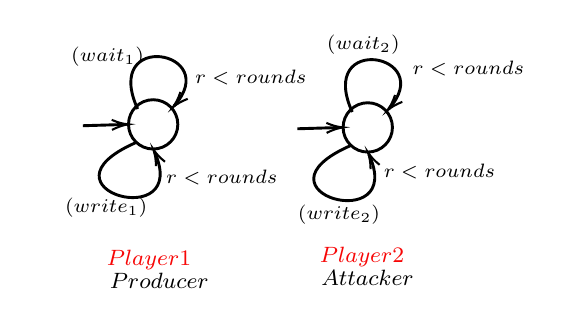
\begin{tikzpicture}[x=0.55pt,y=0.55pt,yscale=-1,xscale=1]
%uncomment if require: \path (0,300); %set diagram left start at 0, and has height of 300

%Shape: Circle [id:dp760252948462048] 
\draw   (192.6,79.1) .. controls (192.6,70.15) and (199.85,62.9) .. (208.8,62.9) .. controls (217.75,62.9) and (225,70.15) .. (225,79.1) .. controls (225,88.05) and (217.75,95.3) .. (208.8,95.3) .. controls (199.85,95.3) and (192.6,88.05) .. (192.6,79.1) -- cycle ;
%Curve Lines [id:da3741641705012937] 
\draw    (198.6,69) .. controls (174.84,16.53) and (254.97,30.71) .. (222.62,66.9) ;
\draw [shift={(221.6,68)}, rotate = 313.41] [color={rgb, 255:red, 0; green, 0; blue, 0 }  ][line width=0.75]    (10.93,-3.29) .. controls (6.95,-1.4) and (3.31,-0.3) .. (0,0) .. controls (3.31,0.3) and (6.95,1.4) .. (10.93,3.29)   ;
%Curve Lines [id:da7883550885112647] 
\draw    (197.6,91) .. controls (127.31,121.69) and (234.42,151.4) .. (209.59,96.98) ;
\draw [shift={(208.8,95.3)}, rotate = 63.88] [color={rgb, 255:red, 0; green, 0; blue, 0 }  ][line width=0.75]    (10.93,-3.29) .. controls (6.95,-1.4) and (3.31,-0.3) .. (0,0) .. controls (3.31,0.3) and (6.95,1.4) .. (10.93,3.29)   ;
%Straight Lines [id:da8536170630459327] 
\draw    (162.6,80) -- (190.6,79.16) ;
\draw [shift={(192.6,79.1)}, rotate = 178.28] [color={rgb, 255:red, 0; green, 0; blue, 0 }  ][line width=0.75]    (10.93,-3.29) .. controls (6.95,-1.4) and (3.31,-0.3) .. (0,0) .. controls (3.31,0.3) and (6.95,1.4) .. (10.93,3.29)   ;
%Shape: Circle [id:dp7766834825103327] 
\draw   (51.6,77.1) .. controls (51.6,68.15) and (58.85,60.9) .. (67.8,60.9) .. controls (76.75,60.9) and (84,68.15) .. (84,77.1) .. controls (84,86.05) and (76.75,93.3) .. (67.8,93.3) .. controls (58.85,93.3) and (51.6,86.05) .. (51.6,77.1) -- cycle ;
%Curve Lines [id:da6262481144264533] 
\draw    (57.6,67) .. controls (33.84,14.53) and (113.97,28.71) .. (81.62,64.9) ;
\draw [shift={(80.6,66)}, rotate = 313.41] [color={rgb, 255:red, 0; green, 0; blue, 0 }  ][line width=0.75]    (10.93,-3.29) .. controls (6.95,-1.4) and (3.31,-0.3) .. (0,0) .. controls (3.31,0.3) and (6.95,1.4) .. (10.93,3.29)   ;
%Curve Lines [id:da4372707429069086] 
\draw    (56.6,89) .. controls (-13.69,119.69) and (93.42,149.4) .. (68.59,94.98) ;
\draw [shift={(67.8,93.3)}, rotate = 63.88] [color={rgb, 255:red, 0; green, 0; blue, 0 }  ][line width=0.75]    (10.93,-3.29) .. controls (6.95,-1.4) and (3.31,-0.3) .. (0,0) .. controls (3.31,0.3) and (6.95,1.4) .. (10.93,3.29)   ;
%Straight Lines [id:da6134143403844121] 
\draw    (21.6,78) -- (49.6,77.16) ;
\draw [shift={(51.6,77.1)}, rotate = 178.28] [color={rgb, 255:red, 0; green, 0; blue, 0 }  ][line width=0.75]    (10.93,-3.29) .. controls (6.95,-1.4) and (3.31,-0.3) .. (0,0) .. controls (3.31,0.3) and (6.95,1.4) .. (10.93,3.29)   ;

% Text Node
\draw (179.6,16) node [anchor=north west][inner sep=0.75pt]  [font=\scriptsize]  {$( wait_{2})$};
% Text Node
\draw (176,170.3) node [anchor=north west][inner sep=0.75pt]  [font=\footnotesize]  {$Attacker$};
% Text Node
\draw (175,155.3) node [anchor=north west][inner sep=0.75pt]  [font=\footnotesize,color={rgb, 255:red, 247; green, 6; blue, 6 }  ,opacity=1 ]  {$Player2$};
% Text Node
\draw (7.6,123) node [anchor=north west][inner sep=0.75pt]  [font=\scriptsize]  {$( write_{1})$};
% Text Node
\draw (11.6,24) node [anchor=north west][inner sep=0.75pt]  [font=\scriptsize]  {$( wait_{1})$};
% Text Node
\draw (37,172.3) node [anchor=north west][inner sep=0.75pt]  [font=\footnotesize]  {$Producer$};
% Text Node
\draw (35,157.3) node [anchor=north west][inner sep=0.75pt]  [font=\footnotesize,color={rgb, 255:red, 247; green, 6; blue, 6 }  ,opacity=1 ]  {$Player1$};
% Text Node
\draw (160.6,128) node [anchor=north west][inner sep=0.75pt]  [font=\scriptsize]  {$( write_{2})$};
% Text Node
\draw (236,33) node [anchor=north west][inner sep=0.75pt]  [font=\scriptsize]  {$r< rounds\ $};
% Text Node
\draw (217,101) node [anchor=north west][inner sep=0.75pt]  [font=\scriptsize]  {$r< rounds\ $};
% Text Node
\draw (93,39) node [anchor=north west][inner sep=0.75pt]  [font=\scriptsize]  {$r< rounds\ $};
% Text Node
\draw (74,105) node [anchor=north west][inner sep=0.75pt]  [font=\scriptsize]  {$r< rounds\ $};


\end{tikzpicture}
